\chapter{Υλοποιήσεις}

Λόγω των επιχειρημάτων της προηγούμενης ενότητας, η πλατφόρμα του
\textit{Nostradamus} αναπτύχθηκε πάνω στην τεχνολογία \textit{Kubernetes}, για
\textit{cloud native} λόγους, αλλά και λόγω της εύκολης παρατηρησιμότητας. Με
αυτόν τον τρόπο, η υποδομή που στηρίζει το έργο καθίσταται υψηλά διαθέσιμη, ενώ
οποιεσδήποτε διαταραχές του συστήματος αντιμετωπίζονται και επιλύονται
αυτόνομα, χωρίς ανθρώπινη παρέμβαση. Λόγου χάριν, σε περίπτωση που ένας κόμβος
παρουσιαστεί ώς μη διαθέσιμος ή ένα \textit{container} (ένα κομμάτι κάποιας
εφαρμογής της πλατφόρμας) καταρρεύσει λόγω προσωρινής αστοχίας λογισμικού ή
υπερφόρτωσης πόρων, το σύστημα αναλαμβάνει την αυτόματη επανεκκίνηση του
σχετικού pod ή ακόμα και τη μετεγκατάστασή του σε διαθέσιμο κόμβο, εφόσον
κριθεί αναγκάιο. Η χρήση μηχανισμών όπως το \textit{livenessProbe} και
\textit{readinessProbe} διασφαλίζει ότι οι υπηρεσίες βρίσκονται πάντα σε
λειτουργική κατάσταση και είναι προσβάσιμες μόνο όταν είναι έτοιμες να
εξυπηρετήσουν αιτήματα.

Η επιλογή αυτής της αρχιτεκτονικής επιτρέπει την υλοποίηση κρίσιμων μηχανισμών
αυτοΐασης (\textit{self-healing}) και κλιμάκωσης, οι οποίοι είναι απαραίτητοι
για το περιβάλλον της γεωργίας ακρίβειας, όπου απαιτείται συνεχής διαθεσιμότητα
και άμεση απόκριση σε μεταβολές φορτίου ή αποτυχιών. Παράλληλα, μέσω της
παρατηρησιμότητας (\textit{observability}) που προσφέρει το οικοσύστημα του
\textit{Kubernetes}, όπως η ενσωμάτωση του \textit{Prometheus} και του
\textit{Grafana}, η πλατφόρμα αποκτά δυνατότητα \textit{real-time} επιτήρησης
μετρήσεων, ειδοποιήσεων και ιχνηλασιμότητας των συμβάντων (\textit{tracing}).

\section{Αρχιτεκτονική υποδομή}

Η αρχιτεκτονική υποδομής της πλατφόρμας σχεδιάστηκε, όπως προαναφέρθηκε, με
σκοπό τη μέγιστη επεκτασιμότητα, διαθεσιμότητα και ασφάλεια, αξιοποιώντας
σύγχρονες τεχνολογίες αυτοματισμού και \textit{containerization}. Το υπόβαθρο
της υλοποίησης βασίζεται στο \textit{Kubernetes}, το οποίο στο πλαίσιο αυτό
φιλοξενήθηκε σε περιβάλλον \textit{homelab}, αλλά η φύση του επιτρέπει την
εύκολη και ομαλή μετάβαση σε οποιοδήποτε \textit{cloud provider}. Επίσης,
εφαρμόστηκαν πρακτικές υποδομής ως κώδικα (\textit{Infrastructure as Code}) και
διαχείρισης μέσω \textit{GitOps}.

\subsection{Τοπολογία και ρόλοι κόμβων}

Η υποδομή αποτελείται απο έναν \textit{Kubernetes cluster} με διακριτούς τύπους
κόμβων:

\begin{itemize}
	\item{\textbf{Control plane nodes}: Υπεύθυνοι για τη λειτουργία
	      του \textit{API server}, του \textit{scheduler}, του \textit{controller
		      manager} και του \textit{etcd}}
	\item{\textbf{Worker nodes}: Εκτελούν τα\textit{pods} των εφαρμογών}
\end{itemize}

Ο διακριτός διαχωρισμός είναι θεμελιώδης για την αξιοπιστία και την ασφάλεια
του \textit{cluster}. Έτσι ο έλεγχος παραμένει απρόσβλητος από αστάθειες ή
σφάλματα που προκαλούνται απο εφαρμογές. Με τη σειρά του, το
\textit{controlplane} συνεχίζει να παρακολουθεί και να θεραπεύει pods, ακόμα
και όταν κάποιες εφαρμογές αποτυγχάνουν.

Τα πειράματα της παρούσας εργασίας έγιναν, λοιπόν, σε έναν \textit{Kubernetes
	cluster} φιλοξενούμενο σε περιβάλλον \textit{homelab}, συγκεκριμένα σε
\textit{enterprise server Dell Poweredge r630}. Χρησιμοποιώντας τεχνολογία
\textit{virtualization} όπως το \textit{Proxmox} ο \textit{server} τμήθηκε σε 5
\textit{virtual machines}, τα οποία αποτελούν τον \textit{cluster}, τα 3 εκ των
οποίων αφιερώθηκαν σε \textit{controlplane nodes} (περιττός αριθμός για λόγους
διατήρησης του \textit{quorum}), ενώ τα υπόλοιπα 2 \textit{virtual machines},
με περισσότερους υπολογιστικούς πόρους, καθιστούν τα \textit{worker nodes}.

\section{Ροή δεδομένων σε πραγματικό χρόνο}

\subsection{Πηγές ροής δεδομένων}

Η αξιόπιστη και χαμηλής καθυστέρησης επεξεργασία ροών δεδομένων σε περιβάλλοντα
γεωργίας ακρίβειας προϋποθέτει την ύπαρξη ποικίλων, ετερογενών πηγών δεδομένων
που παρέχουν συνεχή και διαχρονικά κρίσιμη πληροφορία σχετικά με τη φυσική
κατάσταση του αγροτεμαχίου και τις περιβαλλοντικές μεταβλητές. Η παρούσα
πλατφόρμα σχεδιάστηκε ώστε να ενσωματώνει και να επεξεργάζεται δεδομένα σε
πραγματικό χρόνο από πηγές δεδομένων όπως αισθητήρες θερμοκρασίας και υγρασίας
εδάφους ή μετρητές βροχόπτωσης και φωτεινότητας.

\subsection{Τεχνολογίες Streaming}

Στην προηγούμενη ενότητα παρουσιάστηκε το \textit{Apache Kafka} ως το βασικό
μέσο ενδιάμεσης επικοινωνίας μεταξύ των στοιχείων της πλατφόρμας. Σενάρια
\textit{streaming}, όπως αυτό της πλατφόρμας \textit{Nostradamus}, βασίζονται
στο \textit{Kafka} ως τον κεντρικό κόμβο του συστήματος, ο οποίος λειτουργεί ως
η κύρια <<πηγή αλήθειας>> για όλα τα υποσυστήματα. Κάθε γεγονός που συμβαίνει
στο σύστημα καταγράφεται αρχικά στο \textit{Kafka}, και στη συνέχεια κάθε
μικροϋπηρεσία εγγράφεται στο αντίστοιχο <<θέμα>> (\textit{topic}) ώστε να
λαμβάνει μόνο τα μηνύματα που της είναι απαραίτητα. Με αυτόν τον τρόπο
επιτυγχάνεται ο σαφής διαχωρισμός ανάμεσα στη ροή δεδομένων σε πραγματικό χρόνο
και στην κατανάλωση των μηνυμάτων. Συνεπώς, η σωστή σχεδίαση της υποδομής
συλλογής και μεταφοράς δεδομένων έως το \textit{Kafka} είναι κρίσιμη, καθώς από
εκεί και πέρα ο διαμοιρασμός τους στα υπόλοιπα υποσυστήματα γίνεται με απλό και
αποδοτικό τρόπο.

Για το \textit{deployment} του \textit{Kafka} στην πλατφόρμα επιλέχθηκε το
μοτίβο του \textit{Kubernetes Operator}, με στόχο την υψηλή διαθεσιμότητα, την
ανθεκτικότητα σε αστοχίες και την αυτοματοποιημένη διαχείριση του κύκλου ζωής
του συστήματος. Συγκεκριμένα, χρησιμοποιήθηκε ο \textit{Strimzi Kafka
	Operator}, ο οποίος παρέχει πλήρη αυτοματοποίηση στην εγκατάσταση, ρύθμιση,
κλιμάκωση και αναβάθμιση των brokers, καθώς και στη διαχείριση των
\textit{topics} και των \textit{users}. Με αυτόν τον τρόπο αξιοποιούνται τα
πλεονεκτήματα του Kubernetes, όπως η ευκολία κλιμάκωσης, η αυτόματη
αποκατάσταση υπηρεσιών και η συνεπής διαχείριση πόρων, εξασφαλίζοντας παράλληλα
σταθερή και αποδοτική λειτουργία της υποδομής ροών. Τέλος, ο \textit{operator}
αυτός επιτρέπει την διαχείριση της υποδομής του \textit{Kafka} μέσω
\textit{GitOps} πρακτικών, γεγονός που ευθυγραμμίζεται με τις υπόλοιπες αρχές
και πρότυπα σχεδίασης της παρούσας εργασίας.

Είναι πλέον καθιερωμένη πρακτική οι αισθητήρες και γενικότερα οι χαμηλής
κατανάλωσης μικροελεγκτές που χρησιμοποιούνται σε υποδομές \textit{IoT} να
αποστέλλουν τα μηνύματά τους μέσω του πρωτοκόλλου \textit{MQTT}, καθώς αυτό
εξοικονομεί ενέργεια και επιτρέπει αποδοτική μετάδοση δεδομένων. Για την
εισαγωγή των μηνυμάτων αυτής της μορφής στο \textit{Kafka} απαιτείται η ύπαρξη
μηχανισμού γεφύρωσης. Στο πλαίσιο αυτό, αξιοποιήθηκε αρχικά το \textit{Strimzi
MQTT bridge}.

Ωστόσο, η ενσωματωμένη υλοποίηση του \textit{Strimzi} δεν υποστηρίζει ασφαλή
μεταφορά μέσω \textit{MQTTs}, γεγονός που αποτελεί κρίσιμο ζήτημα για την
παρούσα πλατφόρμα, δεδομένου ότι οι αισθητήρες βρίσκονται σε εξωτερικά δίκτυα.
Για την επίλυση του προβλήματος, ενσωματώθηκε ένας \textit{EMQX broker}, ο
οποίος λειτουργεί ως ασφαλής πύλη (\textit{secure gateway}) μεταξύ των
εξωτερικών συσκευών και του \textit{Kafka}, παρέχοντας υποστήριξη για
κρυπτογράφηση και μηχανισμούς πιστοποίησης σύμφωνα με τις απαιτήσεις της
αρχιτεκτονικής. Παράλληλα, ο \textit{EMQX broker} παρέχει δυνατότητες
φιλτραρίσματος βάσει των εισερχόμενων \textit{MQTT topics} και αντιστοίχισης
(\textit{mapping}) αυτών σε \textit{Kafka topics}, ώστε να προωθούνται στο
\textit{Kafka} μόνο τα απαραίτητα μηνύματα και να διατηρείται συνεπής η
ονοματολογία και η δομή των θεμάτων στην πλατφόρμα.

\subsection{Παρατηρησιμότητα Streaming}

\subsection{Ανθεκτικότητα και ανοχή σε σφάλματα}

\section{Ένταξη πελάτη}

\begin{figure}[H]
	\centering
	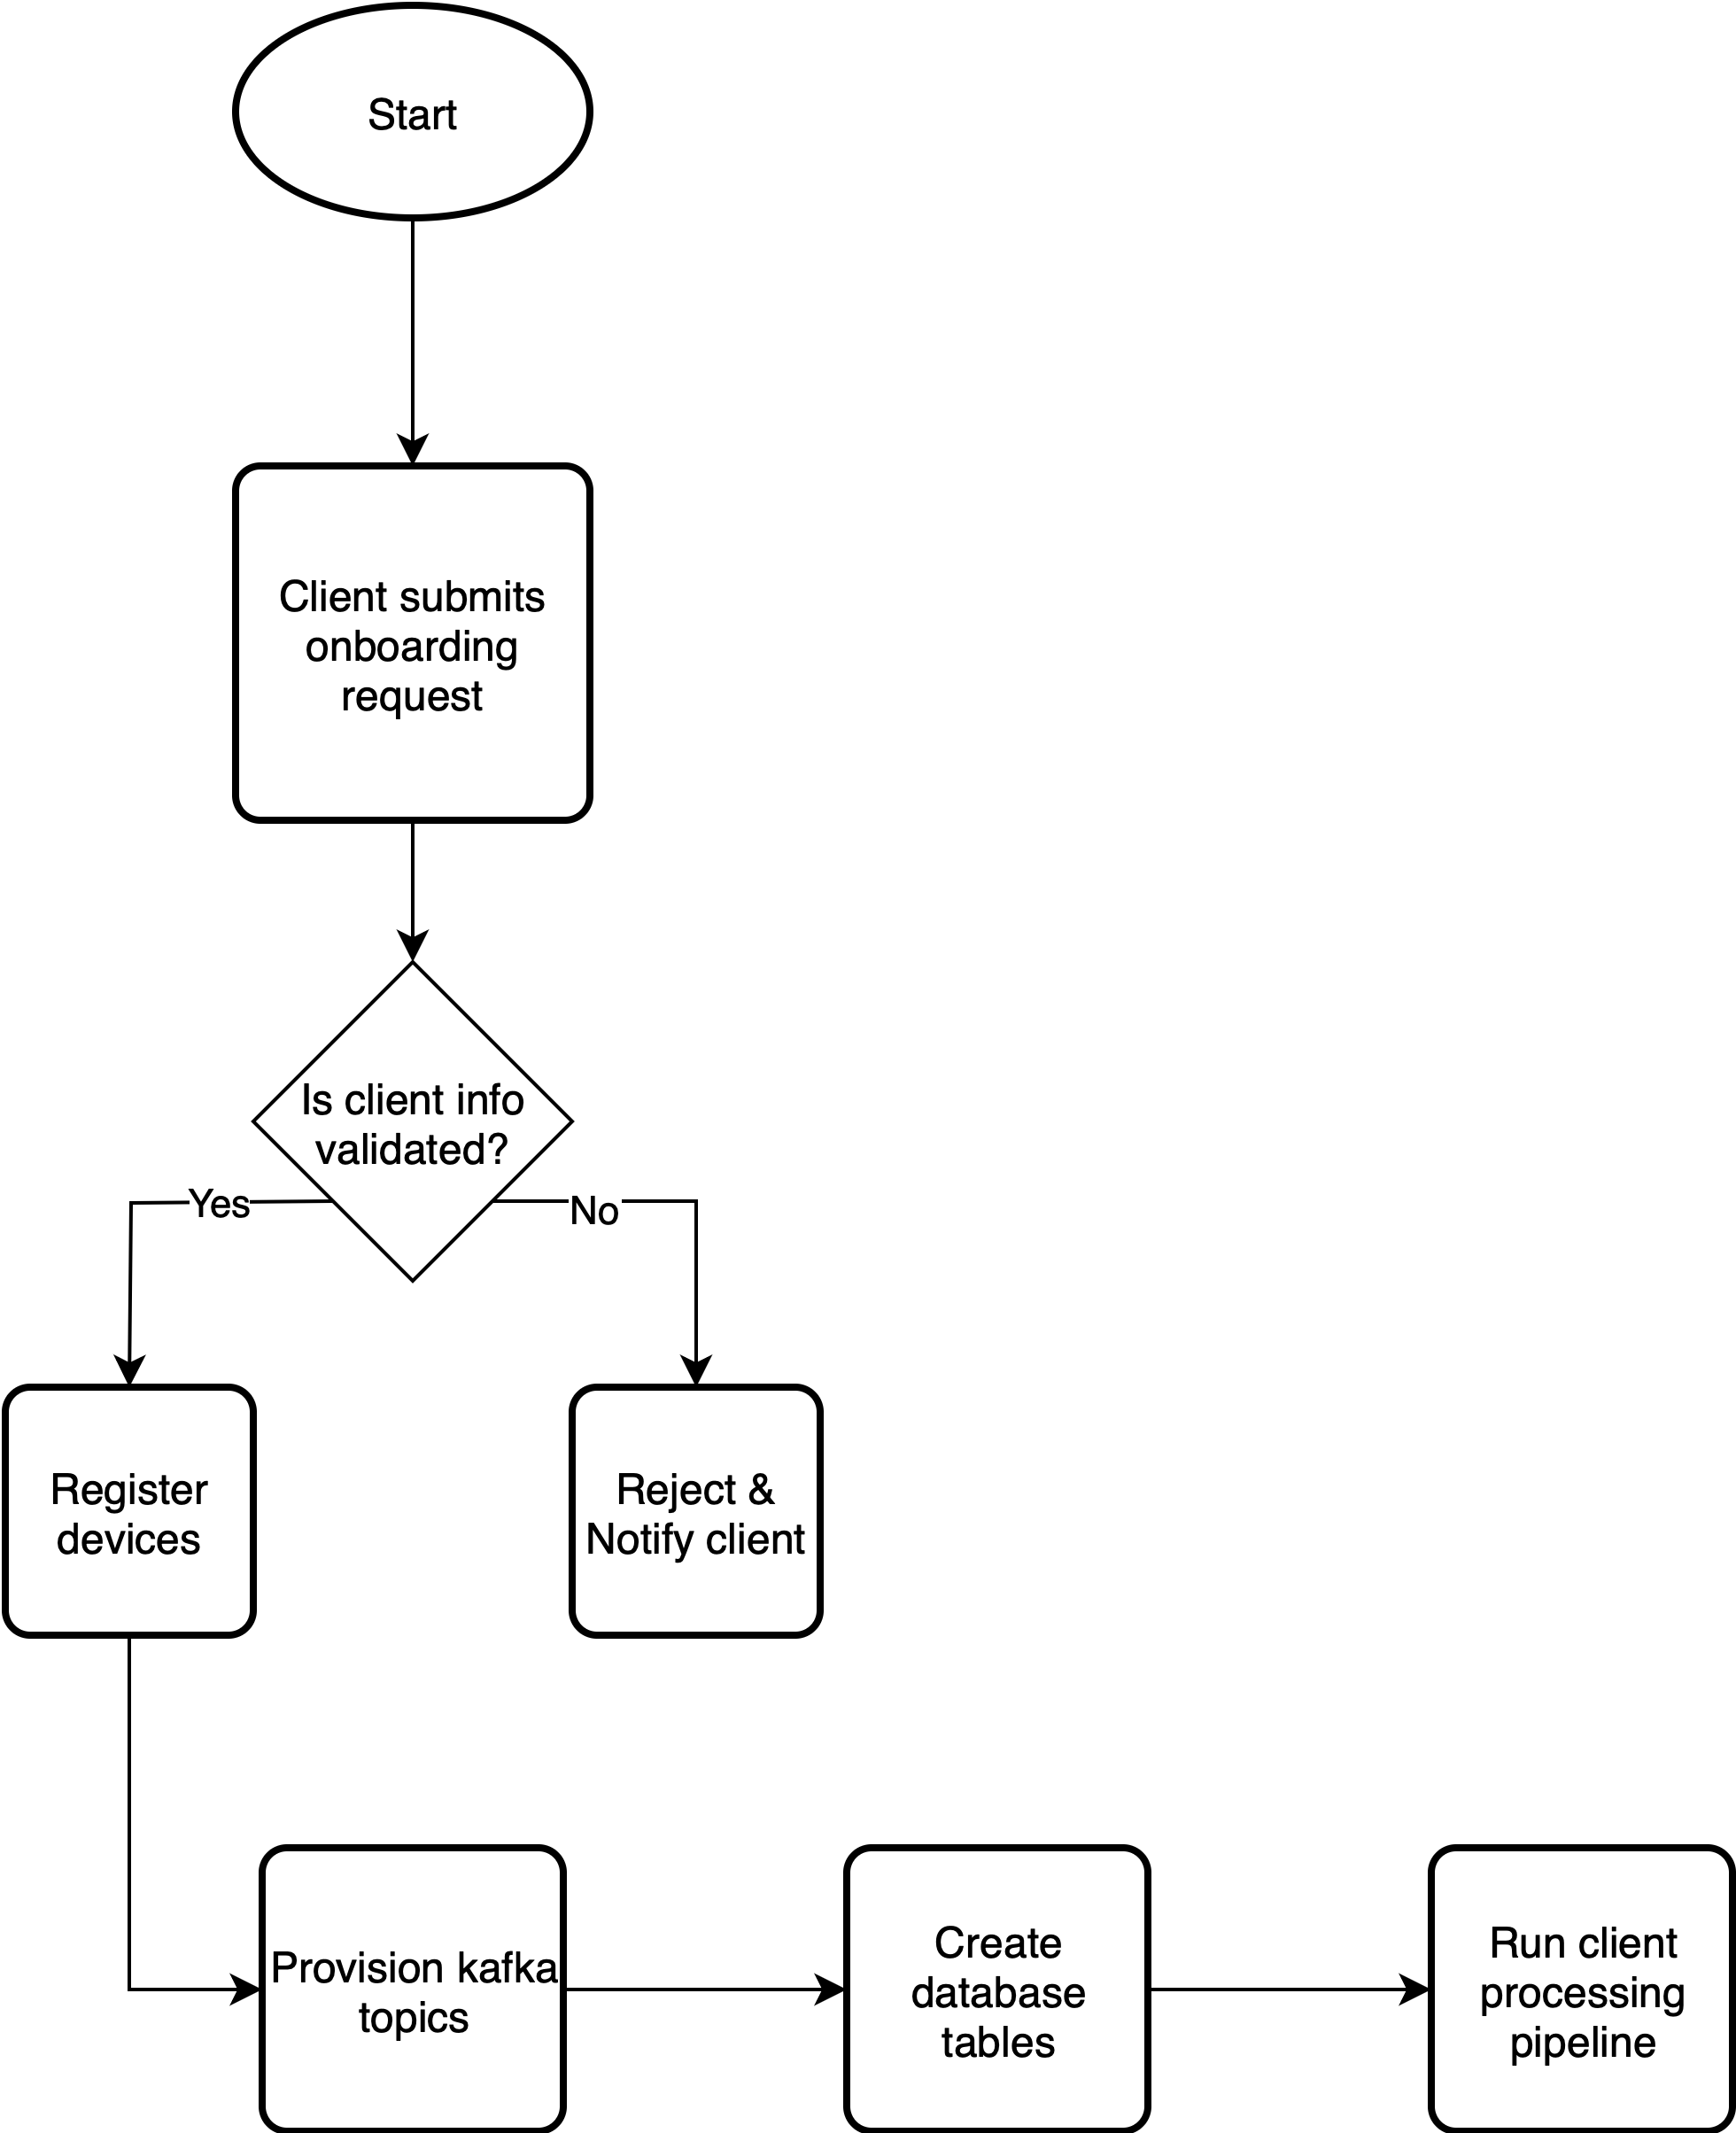
\includegraphics[width=0.7\textwidth]{client-onboarding-process}
	\caption{Διάγραμα δραστηριότητας για τη διαδικασία ένταξης νέου πελάτη}
	\label{fig:client-onboarding-activity}
\end{figure}
